% id: 55-05
% book: 100발100중 3-2 중간 · 01 3-2 중간(삼각비·삼각비의 활용·원과 직선·원주각·부록)
% section: 기출 Best 쌍둥이
% figure: crop:fig-55-05.png
% answer: ③
% answer_source: 답지(빠른정답)
% variant_level: 0 (원본 전사)
% 이 파일은 build.mjs 가 items.json 에서 만든다. 고칠 때는 items.json 을 고친다.
\smash{\raisebox{1.5mm}{\dmkichul{100발100중 3-2 중간 55쪽 05번}}}
\noindent\begin{minipage}[t]{0.58\linewidth}\vspace{0pt}\raggedright 그림에서 $\seg{OM}\perp\seg{AB}$, $\seg{ON}\perp\seg{CD}$이고 $\seg{OM}=\seg{ON}$이다. $\seg{AM}=4$일 때, $\seg{CD}$의 길이는?\end{minipage}\hfill\begin{minipage}[t]{0.4\linewidth}\vspace{0pt}\centering 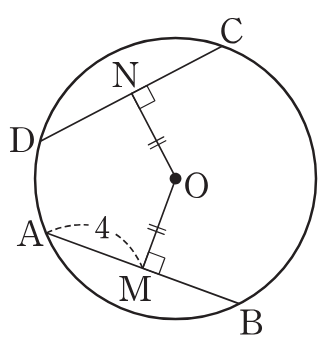
\includegraphics[width=77.7pt]{figures/fig-55-05.png}\end{minipage}\par
\begin{choices32}{$6$}{$7$}{$8$}{$9$}{$10$}\end{choices32}
